\documentclass[12pt, twoside]{article}
\usepackage[letterpaper, margin=1in, head=30pt, headsep=0.1in]{geometry}
\usepackage[english]{babel}
\usepackage[utf8]{inputenc}
\usepackage{amsmath}
\usepackage{amsfonts}
\usepackage{amssymb}
\usepackage{tikz}
%\usetikzlibrary{quotes, angles}

\usepackage{graphicx}
\usepackage{enumitem}
\usepackage{multicol}

\newif\ifmeta
\metatrue %print standards and topics tags

\title{Regents Geometry}
\author{Chris Huson}
\date{October 2021}

\usepackage{fancyhdr}
\pagestyle{fancy}
\fancyhf{}
\renewcommand{\headrulewidth}{0pt} % disable the underline of the header
\raggedbottom


\fancyhead[LE]{\thepage}
\fancyhead[RO]{\thepage \\ Name: \hspace{4cm} \,\\}
\fancyhead[LO]{BECA / Dr. Huson / Geometry 04 Analytic Geometry}

\begin{document}

\subsubsection*{4.5 Linear equations}
The slope of a line: $\displaystyle m=\frac{y_2-y_1}{x_2-x_1}$
\begin{enumerate}
\item Do Now: Find the slope of the line through the points $A(3,4)$, $B(9,8)$.
\begin{flushleft}
  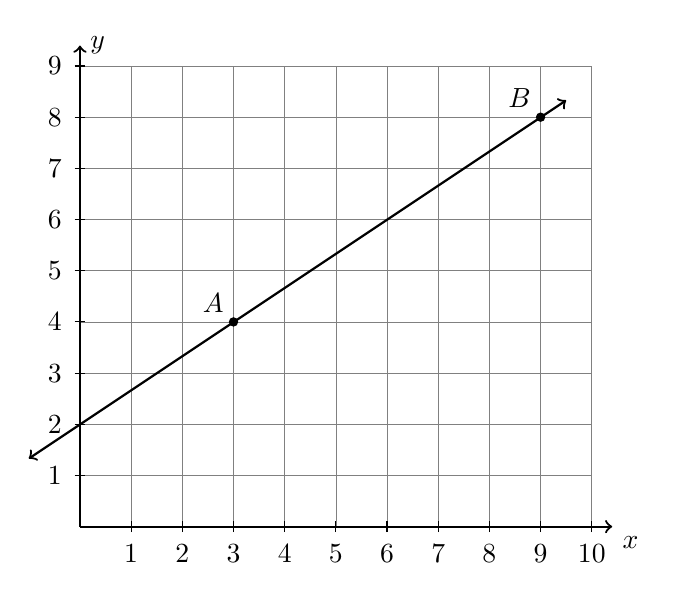
\begin{tikzpicture}[scale=.65]
    \draw [help lines] (0,0) grid (10,9);
    \draw [thick, ->] (0,0) -- (10.4,0) node [below right] {$x$};
    \draw [thick, ->] (0,0)--(0,9.4) node [right] {$y$};
    \foreach \x in {1,...,10}
    \draw[shift={(\x,0)}] (0pt,-3pt)--(0pt,3pt) node[below=5pt] {$\x$};
    \foreach \y in {1,...,9}
    \draw[shift={(0,\y)}] (-3pt,0pt)--(3pt,0pt) node[left=5pt] {$\y$};
    \draw [thick, <->] (-1,1.33)--(9.5,8.33);
    \draw [fill] (3,4) circle [radius=0.08] node[above left] {$A$};
    \draw [fill] (9,8) circle [radius=0.08] node[above left] {$B$};
  \end{tikzpicture}
  \end{flushleft}

\subsubsection*{The slope-intercept equation of a line}
$y=mx+b$, where $m$ is the slope and $b$ is the $y$-intercept
\item The line $l$ has the equation $y=\frac{3}{2}x-1$. 
\begin{enumerate}
  \item Write down it's slope and $y$-intercept. \hspace{2cm} $m=$
  \hspace{2cm} $b=$
  \item Is the point $(4, 4)$ on the line $l$? Justify your answer.
\end{enumerate}
\vspace{2cm}

\item A line is shown on the grid below.
\begin{multicols}{2}
\begin{enumerate}
  \item Write down it's slope, $y$-intercept.\\ $m=$
  \hspace{2cm} $b=$
  \vspace{0.25cm}
  \item Write down the equation of the line.
  \vspace{1cm}
  \item State the coordinates of the point $P$.
\end{enumerate}
  \begin{center}
  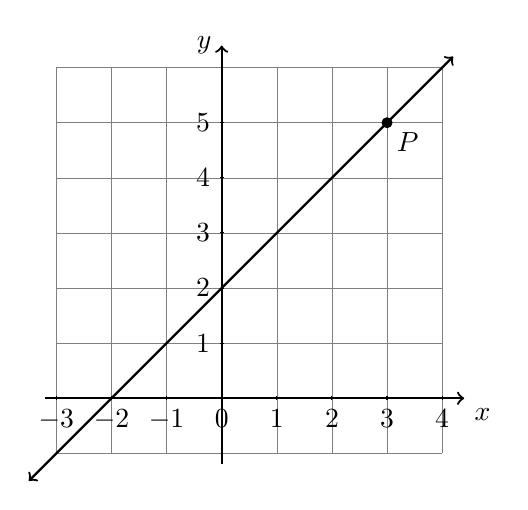
\begin{tikzpicture}[scale=0.7]
    \draw [help lines] (-3,-1) grid (4,6);
    \draw [thick, ->] (-3.2,0) -- (4.4,0) node [below right] {$x$};
    \draw [thick, ->] (0,-1.2)--(0,6.4) node [left] {$y$};
    \foreach \x in {-3, -2, ..., 4} \draw (\x cm,1pt) -- (\x cm,-1pt) node[anchor=north] {$\x$};
    \foreach \y in {1, 2, 3, 4, 5} \draw (1pt,\y cm) -- (-1pt,\y cm) node[anchor=east] {$\y$};
    \draw [thick, <->] (-3.5,-1.5) -- (4.2,6.2);
    \fill (3,5) circle[radius=0.1] node[below right]{$P$};
  \end{tikzpicture}
  \end{center}
\end{multicols}

\newpage
\item Draw a straight line through the points $A$ and $B$ shown on the grid below.
\begin{multicols}{2}
\begin{enumerate}
  \item Write down the line's $y$-intercept.\\ $b=$
  \vspace{0.25cm}
  \item Write down the slope of the line.\\ $m=$
  \vspace{0.25cm}
  \item Write down the equation of the line.
\end{enumerate}
  \begin{center} %4 quadrant regents grid w T-Chart
  \begin{tikzpicture}[scale=0.8]
    %\draw [help lines] (-3,-2) grid (4,6);
    \draw [thick, ->] (-3.2,0) -- (5.4,0) node [below right] {$x$};
    \draw [thick, ->] (0,-1.2)--(0,6.4) node [left] {$y$};
    \foreach \x in {-2, -1, ..., 5} \draw (\x cm,1pt) -- (\x cm,-1pt) node[anchor=north] {$\x$};
    \foreach \y in {1, 2, 3, 4, 5} \draw (1pt,\y cm) -- (-1pt,\y cm) node[anchor=east] {$\y$};
    %\draw [thick, <->] (-3.5,-1.5) -- (4.2,6.2);
    \fill (0,4) circle[radius=0.1] node[above right]{$A (0,4)$};
    \fill (4,2) circle[radius=0.1] node[above right]{$B (4,2)$};
  \end{tikzpicture}
  \end{center}
\end{multicols}
\vspace{1.5cm}

\item Find the coordinates of the midpoint $M$ of $\overline{RS}$, $R(-3,7)$ and $S(5,2)$. Mark and label it on the graph.
  \begin{flushright}
    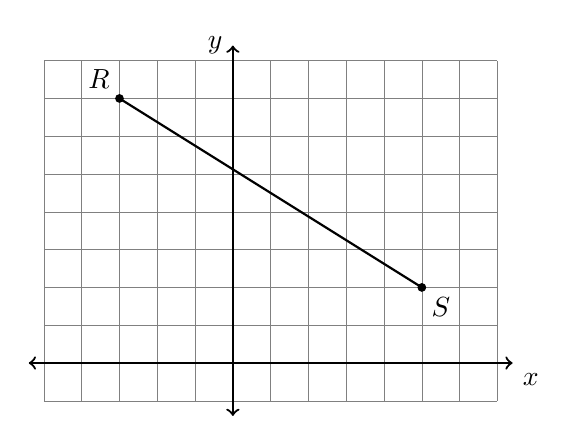
\begin{tikzpicture}[scale=.48]
      \draw [help lines] (-5,-1) grid (7,8);
      \draw [thick, <->] (-5.4,0) -- (7.4,0) node [below right] {$x$};
      \draw [thick, <->] (0,-1.4)--(0,8.4) node [left] {$y$};
      \draw [thick] (-3,7)--(5,2);
      \draw [fill] (-3,7) circle [radius=0.1] node[above left] {$R$};
      \draw [fill] (5,2) circle [radius=0.1] node[below right] {$S$};
    \end{tikzpicture}
  \end{flushright}

\item Point $P$ partitions $\overline{MN}$, $M=-5$ and $N=7$, in the ratio $3:1$. Find the value of point $P$. Mark and label $P$ on the graph. \\[1cm]
  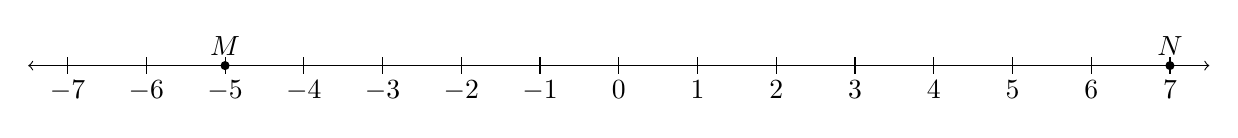
\begin{tikzpicture}
    \draw [<->] (-7.5,0)--(7.5,0);
    \foreach \x in {-7,...,7} %2 leading for diff!=1
      \draw[shift={(\x,0)},color=black] (0pt,-3pt) -- (0pt,3pt) node[below=5pt]  {$\x$};
      \draw [fill] (-5,0) circle [radius=0.05] node[above] {$M$};
      \draw [fill] (7,0) circle [radius=0.05] node[above] {$N$};
  \end{tikzpicture}
  
\end{enumerate}
\end{document}



